\documentclass{article}

\usepackage{stmaryrd}
\usepackage{amsmath}
\usepackage{fullpage}
\usepackage{graphicx}

\begin{document}

\newcommand{\etrans}[1]{\mathcal{E} \llbracket #1 \rrbracket}
\newcommand{\etranst}[1]{\mathcal{E}_t \llbracket #1 \rrbracket}
\newcommand{\etransf}[1]{\mathcal{E}_{f} \llbracket #1 \rrbracket}
\newcommand{\dtrans}[1]{\mathcal{D} \llbracket #1 \rrbracket}
\newcommand{\ttrans}[1]{\mathcal{T} \llbracket #1 \rrbracket}
\newcommand{\strans}[1]{\mathcal{S} \llbracket #1 \rrbracket}
\newcommand{\cf}[1]{\mbox{CF}(#1)}
\newcommand{\trans}[1]{\llbracket #1 \rrbracket}

\newcommand{\unr}{\texttt{UNR}}
\newcommand{\bad}{\texttt{BAD}}
\newcommand{\any}{\texttt{Any}}
\newcommand{\ok}{\texttt{Ok}}

\section{Grammars}

In the following, $D$ is a data constructor, $f$ a function symbol and we consider them as strings. $n$ represents an integer.

\subsection{$\mathcal{H}$: Haskell subset}
Our source language $\mathcal{H}$ is defined below. Note that $\lambda$ abstractions and case expressions can appear anywhere in the code.

assert $(e,c)$ in $e'$ means that if $e$ does not satisfy the contract $c$ then the compiler should return $\BAD$ and otherwise execute $e'$. % TODO return bad? Not really...

$e$ `satisfies` $c$ is a boolean expression which is True iff the expression $e$ satisfies the contract $c$ in the current context. % TODO we talk about cotnract satisfaction in the first paragraph!



\begin{center}
\begin{array}{rclr}
  u,e &:=& x \mid f \mid \lambda x.~e \mid e~e \mid D(e,\dots,e) \mid \bad \mid n \mid e \mbox{ `satisfies` } c \mid \mbox{assert } (e,c) \mbox{ in } e  & (Expression)\\
  &\mid& \mbox{case } e \mbox{ of } [(p_i,e_i)] \mid \cf{e}&\\
  p &:=& \Delta,p \mid T,p \mid f \in c,p \mid \epsilon & (Program)\\
  \Delta &:=& d \mid opaque(d) & (Defintion~and~scope)\\
  d &:=& f~x_1 \dots x_n ::: c = e \mid f~x_1 \dots x_n ::: c = \mbox{ case } e \mbox{ of } [(pat_i,e_i)] & (Definition)\\
  T &:=& \mbox{data } x = DCons  & (Data~type~definition)\\ %TODO make type clearer
  DCons &:=& \epsilon \mid D ; DCons \mid D ::: c ; DCons & (List~of~data~constructors)\\
  pat &:=& D(x_1,\dots,x_n) & (Pattern)\\
\end{array}
\end{center}

\subsection{$\mathcal{H'}$: $\lambda$-lifted haskell subset}
This language is as expressive as $\mathcal{H}$ but contains fewer constructs. Compared to $\mathcal{H}$ the restrictions are:
\begin{itemize}
  \item No $\lambda$, ie every $\lambda$ is lifted to a function definition at the toplevel
  \item No case expressions which are lifted out to the toplevel (ie pattern matching is only possible for a function declaration)
  \item No $assert$ which are syntactic sugar for case expressions
\end{itemize} % TODO describe preprocessing.
From now on, expressions will always refer to $\mathcal{H'}$ expressions.

\begin{center}
\begin{array}{rclr}
  u,e &:=& x \mid f \mid e~e \mid D(e,\dots,e) \mid \bad \mid n \mid e \mbox{ `satisfies` } c \mid \cf{e} & (Expression)\\
  p &:=& \Delta,p \mid T,p \mid f \in c,p \mid \epsilon & (Program)\\
  \Delta &:=& d \mid opaque(d) & (Defintion~and~scope)\\
  d &:=& f~x_1 \dots x_n ::: c = e\mid f~x_1 \dots x_n ::: c = \mbox{ case } e \mbox{ of } [(pat_i,e_i)] & (Definition)\\
  T &:=& \mbox{data } x = DCons  & (Data~type~definition)\\ %TODO make type clearer
  DCons &:=& \epsilon \mid D ; DCons \mid D ::: c ; DCons & (List~of~data~constructors)\\
  pat &:=& D(x_1,\dots,x_n) & (Pattern)\\
\end{array}
\end{center}

For the moment we consider data constructors to be saturated, ie fully applied (hence the special application syntax).
That makes defining $\dtrans{}$ less painful, because we avoid a quadratic number (in the arity of the data contrustors) of axioms. cf $S_4$ below, for example.

\subsection{From $\mathcal{H}$ to $\mathcal{H'}$}
\subsubsection{Step 1: $assert$}
We translate every expression $e = \mbox{assert } (e_c,c) \mbox{ in } e'$ in $\mbox{case } e_c `satisfies` c \mbox{ of } True -> e' | False -> \bad$.
\subsubsection{Step 2: $\lambda-lifting$}
GHC's API can do that.
\subsubsection{Step 3: $case$ lifting}
...


\subsection{FOL}
\begin{center}
\begin{array}{rclr}
  t &:=& x \mid \mbox{app}(t_1,t_2) \mid D(t,\dots,t) \mid f \mid n \mid \bad \mid \unr \mid \mbox{CF}(t) & (Term)\\
  \phi &:=& \forall x.\phi \mid \phi \to \phi \mid \lnot \phi \mid \phi \lor \phi \mid \phi \land \phi \mid true \mid t=t \mid \mbox{CF}(t)& (Formula)\\
\end{array}
\end{center}

We always give the following equations to define crash-freeness:
$$\cf{\unr}, \lnot \cf{\bad}, \forall f,x~\cf{f} \land \cf{x} \implies \cf{app(f,x)}$$
Note that it's only the equation we \textit{always} give, but there some other equations that will arise from the translations below.
It does not follow exactly the semantics given by the popl paper, but we hope it'll be a sufficient approximation!

\subsection{Contracts}
\begin{center}
\begin{array}{rclr}
  c &:=& x:c_1 \to c_2\\
  &\mid& (c_1,c_2) \\
  &\mid& \{ x \mid e \}\\
  &\mid& c_1 \land c_2 \\
  &\mid& c_1 \lor c_2 \\
\end{array}
\end{center}

Semantics of contract satisfaction (exactly the same as in the POPL paper):
\begin{center}
\begin{array}{rcl}
  e \in \{x \mid p \} &\iff& e \mbox{ diverges or } p[e/x] \not \to^\star \{\bad,False\}\\
  e \in x:t_1 \to t_2 &\iff& \forall e_1 \in t_1, (e~e_1) \in t_2[e_1/x]\\
  e \in (t_1,t_2) &\iff& e \mbox{ diverges or } (e \to^\star (e_1,e_2) \mbox{ and } e_1 \in t_1, e_2 \in t_2)\\
  e \in c_1 \land c_2 &\iff& e \in c_1 \mbox{ and } e \in c_2\\
  e \in c_1 \lor c_2 &\iff& e \in c_1 \mbox{ or } e \in c_2\\
\end{array}
\end{center}

\section{CF-ness and unreachability}
\subsection{CF-ness}
In the POPL paper, CF was introduced in the contract satisfaction
semantics because it was required in order to define the
wrapping. Given that we do not use any wrapping, we can make a
separation between crash-freeness and predicate satisfaction now, as
shown in the contracts semantics, with the special syntax.

It leads to some tricky cases:

Assume a reasonable definition of $add$. Then, this contract does not
hold.
$$add ::: a:\{ x \mid True \} \to \{ y \mid True \} \to \{ z \mid z
\geq a \}$$

Why? Because now that we have removed crash-freeness, we can have $x$
and $y$ instantiated to $\bad$. And then, $ add~x~y \geq z $ becomes
$\bad$. Or the semantics say that the predicate should not evaluate to
$\bad$. 

Now, the correct contract is:
$$add ::: a:\{ !x \mid cf(x) \} \to \{ !y \mid cf(y) \} \to \{ !z \mid z
\geq a \}$$


\section{Translation}
We define several translations: $\etrans{},\dtrans{},\ttrans{},\strans{},\trans{}$.
\begin{center}
\begin{array}{rclr}
  \etrans{} &::& Expression \to (Term,FOF)\\
  \dtrans{} &::& Definition \to \{ FOF \}\\
  \ttrans{} &::& Data~type  \to \{ FOF \}\\
  \strans{} &::& Expression \to Contract \to \{ FOF \}\\
  \trans {} &::& Program    \to \{ FOF \}\\
\end{array}
\end{center}

\subsection{$\etrans{}$}
$\etrans{e}$ is a pair (term,formula), the only tricky translations is
for satisfies.  We write $\etranst{}$ and $\etransf{}$ the projection
of $\etrans{}$ on the first and second component.

\begin{eqnarray}
\etrans{x} &=& (x,\emptyset)\\
\etrans{f} &=& (f,\emptyset)\\
\etrans{e_1~e_2} &=& (app(\etranst{e_1},\etranst{e_2}),\etransf{e_1} \cup \etransf{e_2})\\
\etrans{D(e_1,\dots,e_n)} &=& (D(\etranst{e_1},\dots,\etranst{e_n}),\cup_{1 \leq i \leq n} \etransf{e_i})\\
\etrans{\bad} &=& (\bad,\emptyset)\\
\etrans{n} &=& (n,\emptyset)\\
\etrans{e \mbox{ `satisfies` } c} &=& (\etranst{e},\etransf{e} \cup \forall x. \strans{x \in c} \leftrightarrow x~`satisfies`~c = True)\\
\etrans{\cf{e}} &=& \cf{e}\\
\end{eqnarray}

TODO: take car of the FV in c for satisfies.
As usual, we use left associativity.

\subsection{$\ttrans{}$}
$\ttrans{T}$ is a set of first-order formulae which we break down in five parts:
$\ttrans{\mbox{data } T = D_1 ; \dots ; D_n} = S_1 \cup S_2 \cup S_3 \cup S_4 \cup S_5$.

First, for each $D_i$ of arity $n_i$ we introduce selectors $sel_{k,D_i}$, which are projections of $D_i(x_1,\dots,x_n_i)$ on its $k$-th component:
$$S_1 := \{ \forall x_1,\dots,x_{n_i} . \bigwedge_{1 \leq j \leq n} sel_{j,D_i}(D_i(x_1,\dots,x_{n_i})) = x_j \mid 1 \leq i \leq n \}$$

For each pair of different constructors $D_i,D_j$, we state that they can never map to the same value: 
$$S_2 := \{ \forall x_1,\dots,x_{n_i}~\forall y_1,\dots,y_{n_j} . D_i(x_1,\dots,x_{n_i}) \neq D_j(y_1,\dots,y_{n_j}) \mid 1 \leq i < j \leq n \}$$

Then, we have to give crash-freeness conditions for each $D_i$:
$$S_3 := \{ \forall x_1,\dots,x_{n_i} . (\cf{x_1} \land \dots \land \cf{x_{n_i}} \leftrightarrow \cf{D_i(x_1,\dots,x_{n_i})}) \mid 1 \leq i \leq n \}$$
Note that we have an equivalence in the case of a data constructor whereas we only have an (direct) implication for functions. It's because a function, due to laziness, could not use all its arguments. For example, $fst (1,BAD)$ is crash-free but its arguments aren't.

We also have to say that none of the $D_i$ is unreachable:
$$S_4 := \{ D_i(x_1,\dots,x_n) = \unr \to x_1 = \unr \lor \dots \lor x_n = \unr \mid 1 \leq i \leq n \}$$
NB: We first started with $S_4 := \{ D_i \neq \unr \mid 1 \leq i \leq n \}$, but we couldn't prove that the (add x y), defined with peano integers, satisfied ($x=0 \to y=0 \to add~x~y=0$). It's also bizarre to state that the function was $\unr$ but not its application.

Finally, we give contracts to each data constructors. It is the contract $c$ specified by the user. If no contract is given for a specific data constructor, then we assume that the contract is $\ok \to \dots \to \ok$.
We write the contract $c$ as $c_1 \to \dots \to c_{n_i}}$
$$S_5 := \{ \forall x_1,\dots,x_{n_i} \strans{D_i(x_1,\dots,x_{n_i}) \in c} \leftrightarrow \bigwedge_{1 \leq i \leq n_i} \strans{x_i \in c_i} \mid 1 \leq i \leq n \}$$

\subsection{$\dtrans{}$}
$\dtrans{d}$ is a set first-order formula.

\begin{eqnarray}
\dtrans{f~\overline{x} = e} &=& \forall x_1 \dots x_n.\etranst{f~x_1 \dots x_n} = \etranst{e} \cup \etransf{e}\\
\dtrans{f~\overline{x} = \mbox{case } e \mbox{ of } [D_i(\overline{z}) \mapsto e_i]} &=& \forall x_1 \dots x_n.(\bigwedge_i (\forall \overline{z}~\etranst{e} = \etranst{D_i(\overline{z})} \to \etranst{f~\overline{x}} = \etranst{e_i})\\
&& \land \etranst{e} = \bad \to \etranst{f~x_1 \dots x_n} = \bad)\\ 
&& \land ((\bigwedge_i e \neq D_i(sel_{1,D_i}(e),\dots,sel_{n_i,D_i}(e)) \land \etranst{e} \neq \bad)\\
&& ~~\to \etranst{f~x_1 \dots x_n} = \unr)\\
&& \cup \etransf{e}
\end{eqnarray}

Note that in those equations, there is no $\etransf{f~x_1 \dots x_n}$ because it is always the empty set.

An alternative to using selectors would be to write something along the line of $\exists y_1,\dots,y_{D_i}. e \neq D_i(y_1,\dots,y_{D_i})$. It is equivalent but the skolemisation process of equinox will anyway turn those existentials in selectors functions. But if we pattern match $D_i$ in two different functions, we would get two different selectors (the same selector with two different names) so it's better (for the efficiency of the proof) to define selectors for each $D_i$ once in for all and use it as much as possible afterwards.

Equation (10) is not restrictive even in the case of laziness because $e$ is always evaluated.

Equation (11) and (12) state that if we have a type mismatch than the code is $\unr$. It should never occur because we're assuming that the code has already been typechecked.


\subsection{$\strans{}$}
$\strans{e \in c}$ is a set of first-order formulae.
\begin{eqnarray}
\strans{e \in \{x \mid u \}} &=& e = \unr \lor (\etranst{u[e/x]} \neq \bad \land \etranst{u[e/x]} \neq False)\\
&& \cup \etransf{e} \cup \etransf{u[e/x]}\\
\strans{e \in x:c_1 \to c_2}  &=& \forall x_1. \strans{x_1 \in c_1} \to \strans{e~x_1 \in c_2[x_1/x]}\\
\strans{e \in c_1 \land c_2} &=& \strans{e \in c_1} \land \strans{e \in c_2}\\
\strans{e \in c_1 \lor c_2} &=& \strans{e \in c_1} \lor \strans{e \in c_2}\\
\end{eqnarray}
$False$ is a data constructor here.

Remark: we follow the semantics of the POPL paper but it's a bit restrictive.
e.g. in equation 14 we could use the alternate semantics (namely B1 in the POPL paper) : 
$$\strans{e \in \{x \mid u \}} = e = \unr \lor (\etrans{u[e/x]} \neq \bad \land \etrans{u[e/x]} \neq False) \cup \etransf{e} \cup \etransf{u[e/x]}$$

\subsection{$\trans{}$}
$\trans{p}$ defines the translation of a program to a theory (a set of FO formulae)

We have to give some semantics to $\cf{}$, $\bad$ and $\unr$, which are given below.

\begin{eqnarray}
\trans{\epsilon} &=& \{ \cf{\unr}, \lnot \cf{\bad}, \forall f,x~\cf{f} \land \cf{x} \implies \cf{app(f,x)} \}\\
\trans{d,p} &=& \dtrans{d} \cup \trans{p}\\
\trans{opaque(d),p} &=& \dtrans{d} \cup \trans{p}\\
\trans{T,p} &=& \ttrans{T} \cup \trans{p}\\
\trans{f \in c,p} &=& \strans{f \in c} \cup \trans{p}\\
\end{eqnarray}

\section{User interaction}

The user provides a program $p$ which consists of functions definition (either opaque or transparent), data types definition and claims that functions satisfies contracts.

Then, for each function definition $d_f := f~x_1 \dots x_n = e$ of a function $f$ that has to satisfy the set of contracts $C_f$, we construct the context $C = p \setminus ( d_f \cup C_f )$, which is basically the program $p$ without the definition of $f$ and the contracts it has to satisfy. 

We then want to check (with equinox) that:
 $$\trans{C} \cup \{ \dtrans{f~x_1 \dots x_n = e[f^\star/f]}, \dtrans{f^\star~x_1 \dots x_n = e[f^\star/f]}, \bigwedge_{c \in C_f} \strans{f^\star \in c} \} \models \bigwedge_{c \in C_f} \strans{f \in c}$$

Which we rewrite as:
 $$\trans{C} \cup \{ \dtrans{f~x_1 \dots x_n = e[f^\star/f]}, \dtrans{f^\star~x_1 \dots x_n = e[f^\star/f]}, \bigwedge_{c \in C_f} \strans{f^\star \in c},  \bigvee_{c \in C_f} \lnot \strans{f \in c} \} \models \bot$$

\subsection{Checking the contracts in the right order}
Here is a little example showing that we should be careful about we
belong to a theory.

Assume that we have a module that contains two functions defintion $f$
and $g$ and two contracts : $f ::: Any \to Ok$ and $g ::: Any \to
Ok$. We assume that those contract do not hold, for example if $f$ is
$not$ and $g$ is $id$.

Now, we want to check $f$'s contract. We take out $f$'s contract,
translate the function definition for $f$ and $g$ and add the contract
satisfation formulae for $g$'s contract.

But, given that $g$'s contract does not hold, we can derive $\bot$ and
then prove that $f$'s contract hold.

Now the user is happy, and does the same thing for $g$'s contract. It
holds too, given that we can also derive $\bot$ for $f$'s contract.

Finally, the user is really happy, but in fact he has proven nothing.


The solution is to only include the formulae that belongs to a
functions that are actually used. For example, to prove $a$'s
contract, we should only include $f$ and $g$ formulae.

\begin{center}
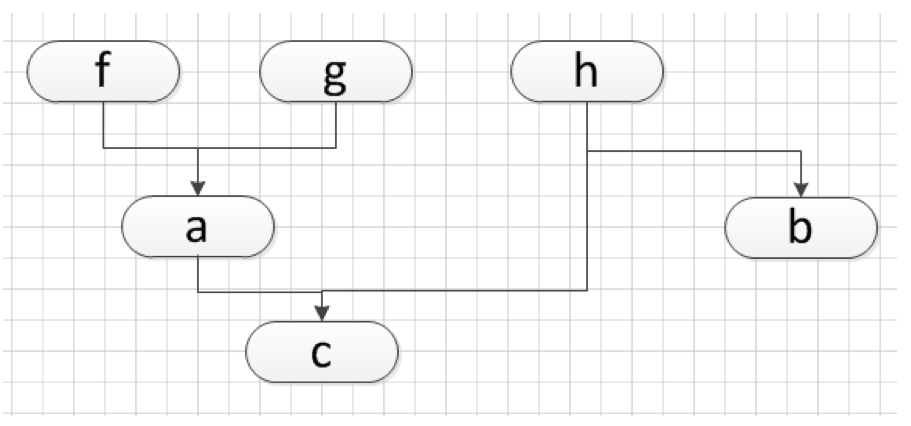
\includegraphics[scale=0.5]{flow.png}
\end{center}



\section{Example}


\subsection{Semantics}
Consider the following program (the integer after a data constructor is its arity):
\begin{verbatim}
data List = Nil 0
          | Cons 2;;

data Bool = True 0
          | False 0;;

copy x = case x of
  | Nil -> x
  | Cons a b -> Cons a (copy b);;

copy ::: a:{!x : True} -> {!y:True};;
\end{verbatim}
The contract states that if we give to copy a crash-free argument $x$, copy will return a crash-free result $y$.
Note that [Just BAD] is not crash-free in our sense, so we can't say anything about it. 


\subsection{Arguments order}
\begin{verbatim}
data Nat = Zero 0
         | Succ 1;;

data Bool = True 0
          | False 0;;

add x y = case x of
        | Zero -> y
        | Succ z -> Succ (add z y);;

isZero x = case x of
         | Zero -> True
         | Succ z -> False;;

not x = case x of
      | True -> False
      | False -> True;;

add ::: a:{!x : isZero x} -> {!y:isZero y} -> {!z: isZero z};;
\end{verbatim}

In the definition of $add$, if we replace $Succ (add z y)$ by $Succ (add y z)$, we can't prove anything which isn't very surprising because we're to do the recursion on the first variable, not on the second one. All the more so that they don't have the same contract.

A lemma stating (+) commutativity would be helpful here.


\subsection{Multiple contracts - Take 1}
We suppose defined datatypes for Nat and Bool, just as in the example above.

\begin{verbatim}
add a b = case a of
  | Zero -> b
  | Succ x -> Succ (add x b);;

mult a b = case a of
  | Zero -> Zero
  | Succ x -> add b (mult x b);;

notZero x = case x of
  | Zero -> False
  | Succ a -> True;;

notZero ::: a:{!x:True} -> {!y: True};;
add  ::: a:{!x: True} -> b:{!y: True} -> {!z: True};;
add  ::: a:{!x: notZero x} -> b:{!y: True} -> {!z: True};;
mult ::: a:{!x: notZero x} -> b:{!y: notZero y} -> {!z: True};;
\end{verbatim}

Equinox diverges when we try to check mult's contract.

The reason stems from that $mult~(Succ~x)~b$ calls recursively
$mult~x~b$ The induction hypothesis says that if $a$ is nonzero and
$b$ is nonzero then the result is $\ok$. But in this case $x$ may be
zero, so the induction hypothesis does not apply immediately. Now, the
theorem prover could do a split on $x$ (either Zero or Succ$\_$) and
in one case the result should follow from the induction hypothesis,
but in the other case we are stuck! Because we don't actually know
that $multp~0~b$ is $\ok$ ($multp$ is the recursive version of the
function, whose contract we assumed but no further defining
equations!)

A possible fix, which is only possible when the function is total is
to write $$f ::: a_1:\{x \mid p_1(x) \} \to \cdots \to a_n:\{x \mid
p_n(x) \}$$ as $$f ::: \ok \to \cdots \to \ok \to \{x \mid
if~(\bidWedge_{i < n} p_i(a_i))~then~p_n(x)~else~True)$$ And know we
can prove $mult$'s contract, but it's not very satisfying.

A stupid fix was to provide defining equations for $multp$ (the same
as for $mult$). Indeed, we could prove that $mult$ satisfied its
contract, but it was trivially true...

Current idea is to unfold the definition a fixed number of times.

\section{De-appification and removed CFness}
\subsection{De-appification}
Instead of always using the $app$ function when doing function
application, we now use directly the function name if it is fully
applied. For example, if $f$ is of arity 2, $f x y$ is now translated
to $f(x,y)$ instead of $app(app(f,x),y)$.  To deal with partially
applied functions, we can use $f\_ptr$ and some extra axioms. 

This transformation makes things much faster for equinox, especially
given that in most cases, function are totally applied.

\end{document}

